\chapter{Réalisation}

\section{Interface graphique}

\subsection{Panneaux et boutons}

Nos panneaux dérivent de la classe \emph{JPanel}, elle-même issue de la classe \emph{Panel}. Cette dernière fournit un composant Container permettant d'accueillir d'autres composants graphiques (sous-panneaux).\\

Le premier panneau (\textbf{panel1}) contient une zone de texte (\emph{JLabel}) afin d'afficher un message d'aide, ainsi qu'un menu déroulant (\emph{JComboBox}) pour le choix des algorithmes. \\

Le panneau central (\textbf{panel2}) est vide au lancement du plugin et son contenu varie en fonction de l'algorithme sélectionné. Par exemple pour l'algorithme Difference of Gaussian, les sous-panneaux sont créés dans la classe \texttt{panelDoG}. Pour cet algorithme, le \textbf{panel2} comprend :
\begin{itemize}
\item \textbf{infoPanel} contenant un \emph{JLabel} indiquant le type d'image requis.
\item \textbf{sigmaPanel} et \textbf{widthNoisePanel} qui contiennent des \emph{JLabel} et \emph{JTextField} afin de créer une zone dans laquelle peut entrer les paramètres nécessaires au déroulement du piquage. 
\item \textbf{debugCropPanel} quand à lui contient deux cases à cocher (\emph{JCheckBox}) pour activer ou non les modes de débogage et de crop. 
\end{itemize}
Les classes \emph{panelImCorr} et \emph{panelDilateDiff} servent à la création des sous panneaux des algorithmes Image Correlation et Dilate Difference respectivement. \\

Le dernier panneau (\textbf{panel3}) comporte quatre boutons (\emph{JButton}) devant répondre aux clics de la souris à l'aide d'un \emph{ActionListener}. \\

Enfin, le panneau principal (\textbf{mainPanel}) contient tous les panels cités précédemment. Sa taille détermine celle de la fenêtre du plugin. \\
Ces quatre panneaux sont crées dans la classe \texttt{PickFrame}, qui hérite de la classe \texttt{JFrame}. \texttt{PickFrame} peut également accéder à des méthodes de la classe \texttt{ActionListener}. 

\subsection{Affichage des résultats}

Lorsque l'utilisateur a coché la case "crop" avant de lancer la procédure de piquage, la classe \texttt{PickFrame} fait appel à la classe \texttt{Cropper} permettant de créer un stack. Les paramètres d'entrée de \texttt{Cropper} sont une \emph{ImagePlus} (image courante du stack) et un tableau de doubles contenant les coordonnées des particules sélectionnées. \\
A partir de ce tableau, la méthode \texttt{crop()} de \texttt{Cropper} fait appel à la méthode \texttt{setRoi()} d'\imj ~afin de retenir une zone carrée autour de la sélection. Cette zone va ensuite être dupliquée et ajoutée au stack sous la forme d'un \emph{ImageProcessor}. \\

Par ailleurs, les résultats de la sélection peuvent être affichés sous la forme d'une \texttt{ResultsTable} si on clique sur le bouton "Show Results". Elle est construite grâce au tableau de doubles cité précédemment, qui est le paramètre d'entrée de la fonction \texttt{generate-} \texttt{CsvFile()}. 

\section{Récupération des paramètres}

Le singleton de la classe \texttt{Attributes} contient une table de hashage (\emph{HashTable}) dans laquelle sont stockés tous les paramètres entrés par l'utilisateur. Ces derniers sont accessibles grâce à des clés et donc réutilisables dans les algorithmes. Le mot-clé  \texttt{synchronized} dans la fonction  \texttt{getInstance()} empêche toute instanciation multiple. 

\section{Algorithmes}

Lorsque l'utilisateur fait le choix d'un algorithme de piquage parmi ceux qui lui sont proposés, cela fait appel à la classe AlgoFactory contenant une méthode switch. Celle-ci permet de récupérer le nom de l'algorithme choisi et d'afficher le panel2 correspondant. \\
Une fois le panel2 chargé, l'appel aux procédures de piquage ne peut se faire que si l'on clique sur les boutons de prévisualisation (Preview) ou d'application à l'ensemble du stack (Apply). Les paramètres entrés par l'utilisateur sont sauvegardés dans la table de hashage grâce à la fonction getInstance() de la classe Attributes, puis récupérés, pour l'algorithme, par la fonction setAttributes() de la classe PanelDoG (pour suivre notre scénario). L'algorithme est ensuite appelé par la méthode sliceSelection(). 










\section{Applications}

Le résultat affiché sur l'image correspond aux positions des particules sur l'image courante ou la dernière image dans le cas d'un stack.
L'utilisateur peut choisir d'afficher un tableau contenant les coordonnées (abscisses, ordonnées et positions dans le stack) des particules sélectionnées et pourra le sauvegarder. \\
De plus, s'il le désire, un stack contenant les particules sélectionnées aux positions obtenus est créé (éliminant les particules trop près du bord de l'image) et affiché.
\begin{figure}[ht]
 \begin{minipage}{.450\linewidth}
  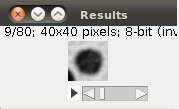
\includegraphics[width=0.75\textwidth]{cropblob.png}  
 % \caption{Difference de Gaussienne (blobs)}
 \end{minipage} \hfill
\begin{minipage}{.450\linewidth}
  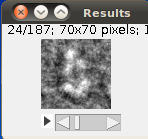
\includegraphics[width=0.5\textwidth]{cropprotDog.png}   
  %\caption{Difference de Gaussienne (protéines)}
 \end{minipage} \hfill
\caption{Exemple d'image formant le stack de particules (blobs et protéines)}
\end{figure}
\subsubsection*{Statistiques}
La Différence de Gaussienne permet d'obtenir les résultats suivant :

\begin{figure}[ht]
 \begin{minipage}{.450\linewidth}
  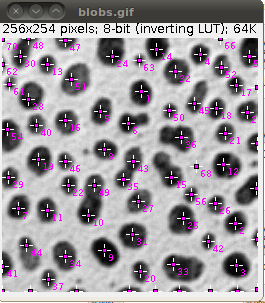
\includegraphics[width=0.75\textwidth]{blobsDog.png}  
 % \caption{Difference de Gaussienne (blobs)}
 \end{minipage} \hfill
\begin{minipage}{.450\linewidth}
  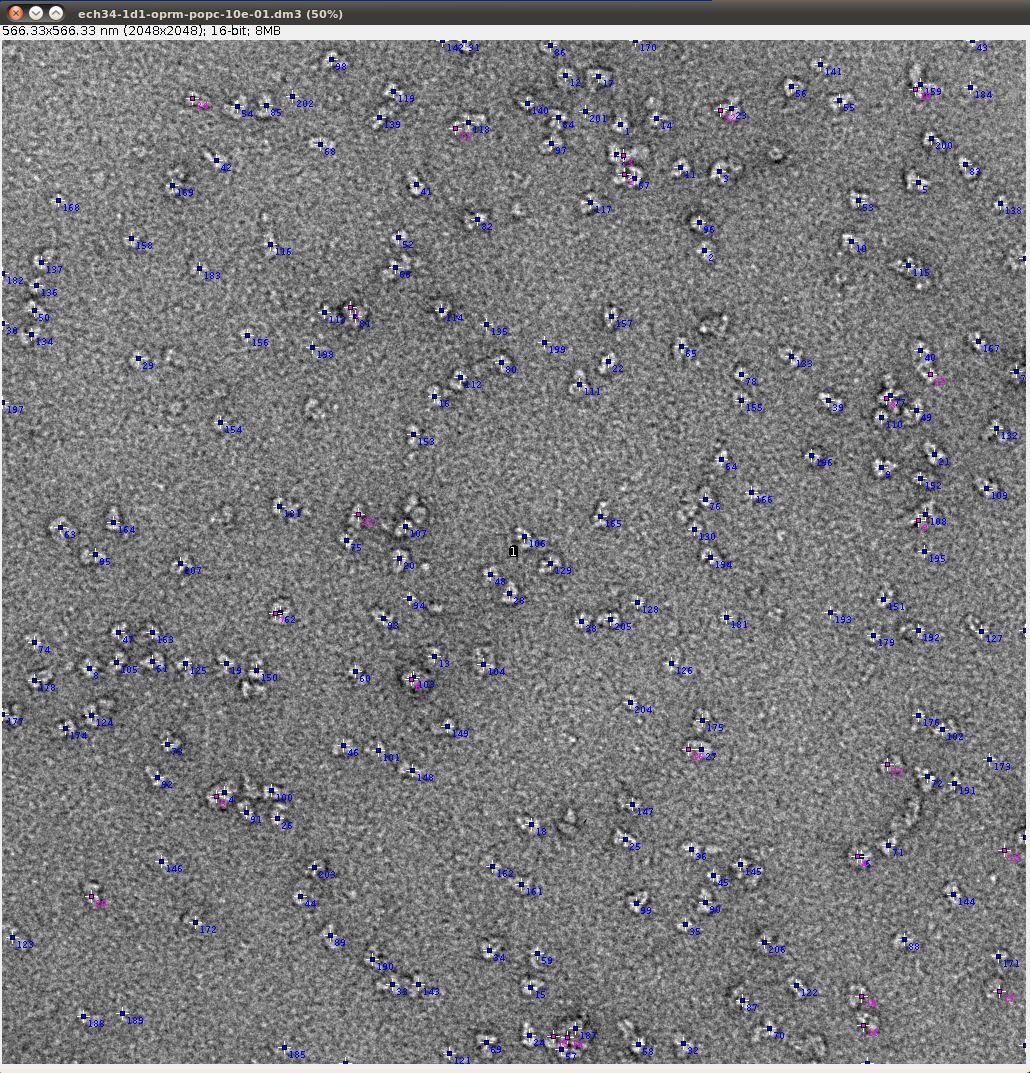
\includegraphics[width=1\textwidth]{protDog.png}   
  %\caption{Difference de Gaussienne (protéines)}
 \end{minipage} \hfill
\caption{Difference de Gaussienne (blobs et protéines)}
\end{figure}
La Différence de dilatation permet d'obtenir les résultats suivant :


%algoFactory
%La présence d'un constructeur privé supprime le constructeur public par défaut.
%De plus, seul le singleton peut s'instancier lui même.

%attributes et algoFact
%
%Il est TRES important.






























